\documentclass[12pt]{exam}
\usepackage[T1]{fontenc}
\usepackage[utf8]{inputenc}
\usepackage[brazil]{babel}
\usepackage{lmodern}
\usepackage{graphicx}
\usepackage[normalem]{ulem}
\usepackage{hyperref}

\footer{}{}{}

\title{}
\date{}

\newcommand{\siheader}{
\begin{center}
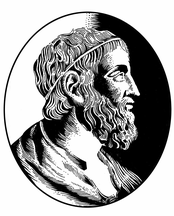
\includegraphics{archi.png}
\vspace{0.5cm}
{\huge Prova de Estágio na Seção de Informática}
\vspace{0.3cm}
\makebox[\textwidth]{Nome:\enspace\hrulefill}
\makebox[\textwidth]{Assinatura:\enspace\hrulefill}
\end{center}
}


\begin{document}
\siheader
\section*{Recomendações}
Para as seções posteriores, se necessário, use:

\subsection*{Credenciais}
\begin{verbatim}
usuário: zelele
senha: zelele123
\end{verbatim}

\subsection*{Tabela de MAC}
\begin{table}[h!]
\begin{tabular}{ |c|c| }
    \hline
    usuário & mac-address \\ \hline
    alopes & \verb+00:de:ad:be:ef:00+ \\ \hline
    gnann & \verb+31:41:59:26:53:58+ \\ \hline
    hcabral & \verb+00:fe:0f:f1:10:ff+ \\ \hline
    milare & \verb+ca:fe:ca:fe:ca:fe+ \\ \hline
    zelele & \verb+ab:bc:cd:de:ef:fg+ \\ \hline
    zemane & \verb+00:de:ad:be:ef:00+ \\ \hline
\end{tabular}
\end{table}

%%% HARDWARE %%%
\section*{Hardware}
\begin{questions}

\question
Montar o computador.

\begin{parts}
\part
Conecte adequadamente as placas.

\part
Conecte adequadamente os periféricos.

\part
Ligue o computador.
\end{parts}

\question
Carregar o sistema Windows já instalado.

\end{questions}
\newpage


%%% WINDOWS %%%
\section*{Windows}
\begin{questions}

\question
Configurar corretamente o teclado.

\question
Verificar o endereço \verb+IP+ do computador e mudar.
\begin{itemize}
    \item Novo IP: \verb+192.168.57.3+
    \item Máscara: \verb+255.255.192.0+
    \item Gateway: \verb+192.168.45.1+
    \item DNS: \verb+143.107.45.1+
\end{itemize}

\question
Instalar a impressora \verb+Borracha+ e imprimir uma página de teste. O
endereço dela na rede é

\begin{quote}
\verb+http://cups.ime.usp.br:631/printers/Borracha+
\end{quote}

e o \textit{driver} que ela usa está na \textit{Área de Trabalho}.

\question
Dadas as credenciais:
\begin{itemize}
\item usuário: \verb+zeprova+
\item senha: \verb+pratiqueatividadesfisicasregularmente+
\end{itemize}

Instalar a versão do navegador \textit{Firefox} disponível na nossa rede
no endereço:
\begin{quotation}
    \verb+\\DONBOT\estagiprova+
\end{quotation}

\question
Instalar a partir do site \url{https://ninite.com/} o \textit{Java}$\ldots$

\question
Instalar o \textit{R}.

\question
Criar o usuário \verb+zemane+ com a senha \verb+zemane123+.

\question
Salve na Área de Trabalho uma lista dos itens de inicialização do Windows. Pode ser texto, imagem ou qualquer formato legível.

\end{questions}
\newpage


%%% LINUX %%%
\section*{Linux}
\begin{questions}

\question
Verificar o endereço \verb+IP+ do computador e mudar para \verb+192.168.57.3+,
com a máscara \verb+255.255.192.0+ e o \verb+gateway+ como \verb+192.168.45.1+
 e \verb+DNS+ como \verb+143.107.45.1+.

\question
Instalar a impressora \verb+Borracha+ e imprimir uma página de teste. O
endereço dela na rede é

\begin{quote}
\verb+http://cups.ime.usp.br:631/printers/Borracha+
\end{quote}

e o modelo dela é \verb+HP 1022+ e o \verb+PPD+ pode ser obtido em:
\begin{quote}
\verb+http://cups.ime.usp.br:631/printers/Borracha.ppd+
\end{quote}

\question
Instalar a versão atualizada do navegador \textit{Chromium}.

\question
Instalar a versão 6 do \textit{Libre Office}

OBS: sugerimos utilizar a versão do \verb+backports+ via gerenciador de pacotes.

\question
Instalar o \verb+PlayOnLinux+ utilizando algum gerenciador de pacotes.
\begin{parts}
\part
Adicionar a arquitetura \verb+i386+ usando os comandos:
\begin{itemize}
    \item{\verb+dpkg --add-architecture i386+}
    \item{\verb+apt update+}
\end{itemize}
\part
Usando o gerenciador de pacotes, instalar \verb+wine32-development+.

\part
Dentro do \verb+PlayOnLinux+, instalar o \textit{Microsoft Pinball}.
\end{parts}

\question
Criar o usuário \verb+zemane+ com a senha \verb+zemane123+.

\question
Logar via \verb+SSH+ no \verb+IP 192.168.57.101+ com o usuário \verb+estag4+
e a senha
\begin{quotation}
    \verb+pratiqueatividadesfisicasregularmente+
\end{quotation}
e cadastrar os endereços \verb+MAC+ fornecidos usando o
comando \verb+novaplaca+.

OBS: sugerimos cadastrar uma a uma.

\question
Reconfigurar o \textit{swap}.
\begin{parts}
\part
Identificar qual partição está utilizando o \textit{swap}.
\part
Desligar o \textit{swap};
\part
Criar um novo \textit{swap} a partir de um arquivo.
\end{parts}

\question
A partir do LVM:
\begin{parts}
\part
Criar um volume físico com a partição que continha o \textit{swap};
\part
Criar um volume lógico a partir do volume físico;
\part
Formatar o volume lógico como \verb+ext4+;
\part
Montá-lo em \verb+/tmp+.
\end{parts}

\end{questions}
\end{document}
